\PassOptionsToPackage{unicode}{hyperref}
\documentclass[aspectratio=1610, captions=tableheading, 11pt]{beamer}
\usepackage{booktabs}
% Load packages you need here
\usepackage{polyglossia}
\setmainlanguage{german}

\usepackage{csquotes}
    

\usepackage{amsmath}
\usepackage{amssymb}
\usepackage{mathtools}
\usepackage[mathrm=sym]{unicode-math}
\usepackage{relsize}

\usepackage[
  locale=DE,                 % deutsche Einstellungen
  separate-uncertainty=true, % immer Fehler mit \pm
  per-mode=reciprocal,       % ^-1 für inverse Einheiten
  % alternativ:
  % per-mode=reciprocal, % m s^{-1}
  % decimal-marker=., % . statt , f�r Dezimalzahlen
]{siunitx}

\usepackage{hyperref}
\usepackage{bookmark}
\usepackage[utf8]{inputenc}

% load the theme after all packages

\usetheme[
  showtotalframes, % show total number of frames in the footline
]{tudo}

% Put settings here, like
\unimathsetup{
  math-style=ISO,
  bold-style=ISO,
  nabla=upright,
  partial=upright,
  mathrm=sym,
}

\usepackage{tikz-feynman}
\usepackage{xfrac}
\usepackage{tikz}
\usetikzlibrary{shapes,arrows}

\tikzstyle{decision} = [rectangle, draw, fill=red!20, 
    text width=15em, text centered, rounded corners, minimum height=2em]
\tikzstyle{block} = [rectangle, draw, fill=blue!20, 
    text width=20em, text centered, rounded corners, minimum height=2em]
\tikzstyle{line} = [draw, -latex']
\tikzstyle{cloud} = [draw, ellipse,fill=red!20, node distance=3cm,
    minimum height=2em]

\setbeamertemplate{caption}{\raggedright\insertcaption\par}

% nur wenn akkurat auf dem Rechner installiert ist:
\setsansfont{Akkurat Light}[
  BoldFont=Akkurat Bold,
]


\author[J. Alameddine]{Jean-Marco Alameddine}
\title{Improvements in the high-energy\\ lepton propagator PROPOSAL}
\date[25.03.2019]{25.03.2019}

\institute[%
  {
\includegraphics[height=0.9\headerheight]{e5b.pdf}}%
]{E5b}

\newcommand\CC{C\nolinebreak[4]\hspace{-.05em}\raisebox{.4ex}{\relsize{-3}{\textbf{++}}}\:}
%\titlegraphic{\includegraphics[height=0.4\textheight]{example-image-a}}

\begin{document}

\begin{frame}
  \maketitle
\end{frame}

%%% Introduction %%%

\begin{frame}{Introduction}
      \begin{itemize}
        \setlength\itemsep{0.5em}
        \item \textbf{PROPOSAL}: Tool to propagate charged leptons
        \begin{itemize}
          \item[$\rightarrow$] MC simulations, multivariate statistics
        \end{itemize}
        \item \textbf{Requirements:} Accuracy, performance
        \item \textbf{Processes:} Energy losses, scattering, decays
        \item Possibility to use \textbf{different parametrizations} $\rightarrow$ Study \textbf{systematic uncertainties}
        \item \CC library with Python bindings
      \end{itemize}
\end{frame}

\begin{frame}{Propagation}
  \Huge
  \begin{align*}
      \frac{\mathrm{d}\sigma}{\mathrm{d}v} \quad \underbrace{\longrightarrow}_{?} \quad \text{energy losses}
  \end{align*}
\end{frame}

\begin{frame}{Propagation}
  \huge
  \begin{align*}
      \underset{\text{continuous losses}}{v < v_\text{cut}} && \underset{\text{stochastic losses}}{v_\text{cut} < v}
  \end{align*}\\
  \vspace{20px}
  \centering
    \Large
  with $v_\text{cut} = \text{min}\left[\sfrac{e_\text{cut}}{E}, v\prime_\text{cut} \right]$
\end{frame}

\begin{frame}{Propagation}
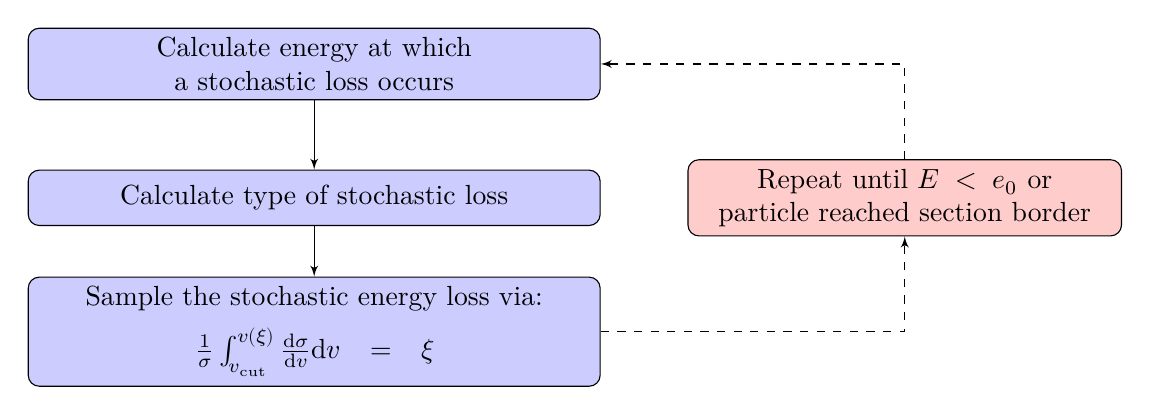
\begin{tikzpicture}[node distance = 1.7cm, auto]
    % Place nodes
    \node [block] (one) {Calculate energy at which a stochastic loss occurs};
    %\node [block, below of=one] (two) {Calculate continuous losses via:\\ \vspace{5px}
 %$- \left\langle \frac{\mathrm{d}E}{\mathrm{d}x} \right\rangle \propto E \int_{v_\text{min}}^{v_\text{cut}} v \frac{\mathrm{d}\sigma}{\mathrm{d}v} \mathrm{d}v$};
    \node [block, below of=one] (two) {Calculate type of stochastic loss};
    \node [block, below of=two] (three) {Sample the stochastic energy loss via:\\\vspace{5px} $\frac{1}{\sigma} \int_{v_\text{cut}}^{v\left(\xi\right)} \frac{\mathrm{d}\sigma}{\mathrm{d}v} \mathrm{d}v = \xi$};
    \node [decision, right of=two, node distance=7.5cm] (repeat) {Repeat until $E < e_0$ or\\ particle reached section border};

    % Draw edges
    \path [line] (one) -- (two);
    \path [line] (two) -- (three);
    %\path [line] (three) -- (four);
    \path [line, dashed] (three) -| (repeat);
    \path [line, dashed] (repeat) |- (one);



\end{tikzpicture}
\end{frame}

\begin{frame}

\begin{figure}
    \centering
    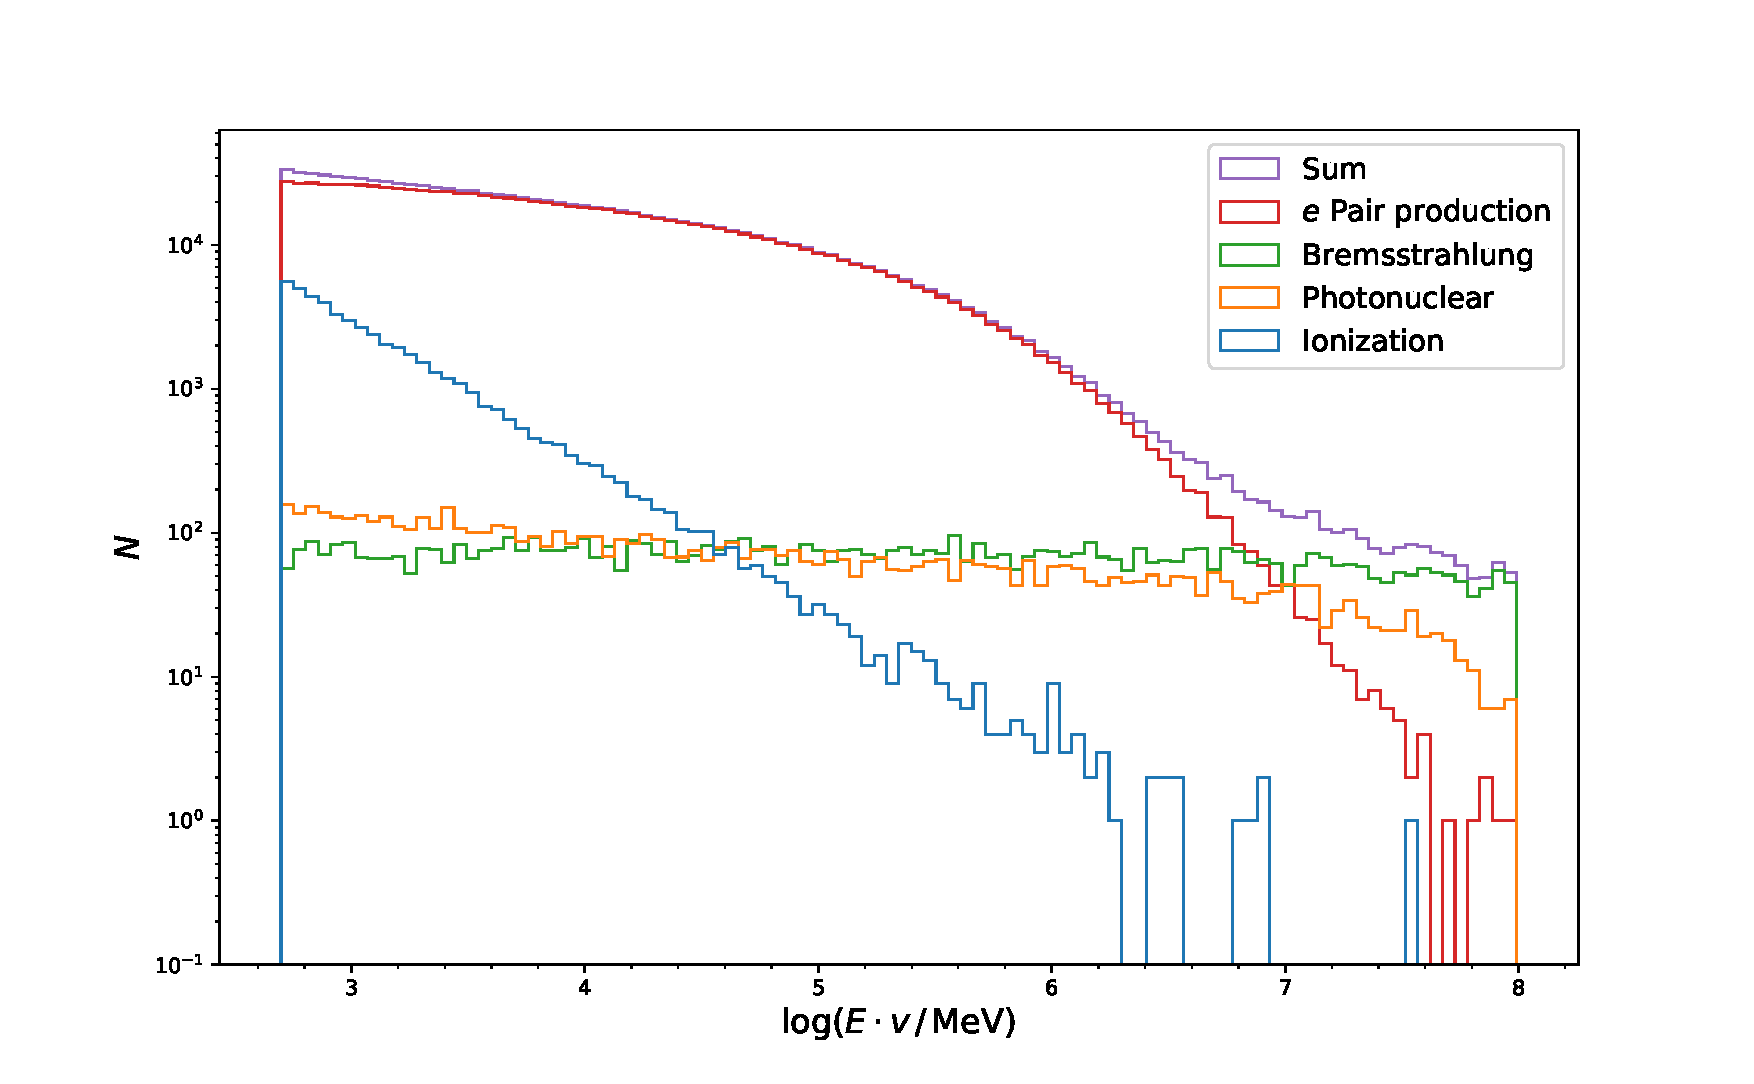
\includegraphics[height=0.85\textheight, trim=1.9cm 0.5cm 1.9cm 2cm,clip=true]{plots/standard.pdf}
    \caption{Propagation of $\num{e4}$ muons with energy $\SI{e8}{\mega\electronvolt}$ through $\SI{100}{\metre}$ of Standard Rock.}
    \label{fig:1}
\end{figure}
\end{frame}

\begin{frame}<presentation:0>[noframenumbering]
\begin{figure}
  \begin{minipage}[c]{0.7\textwidth}
    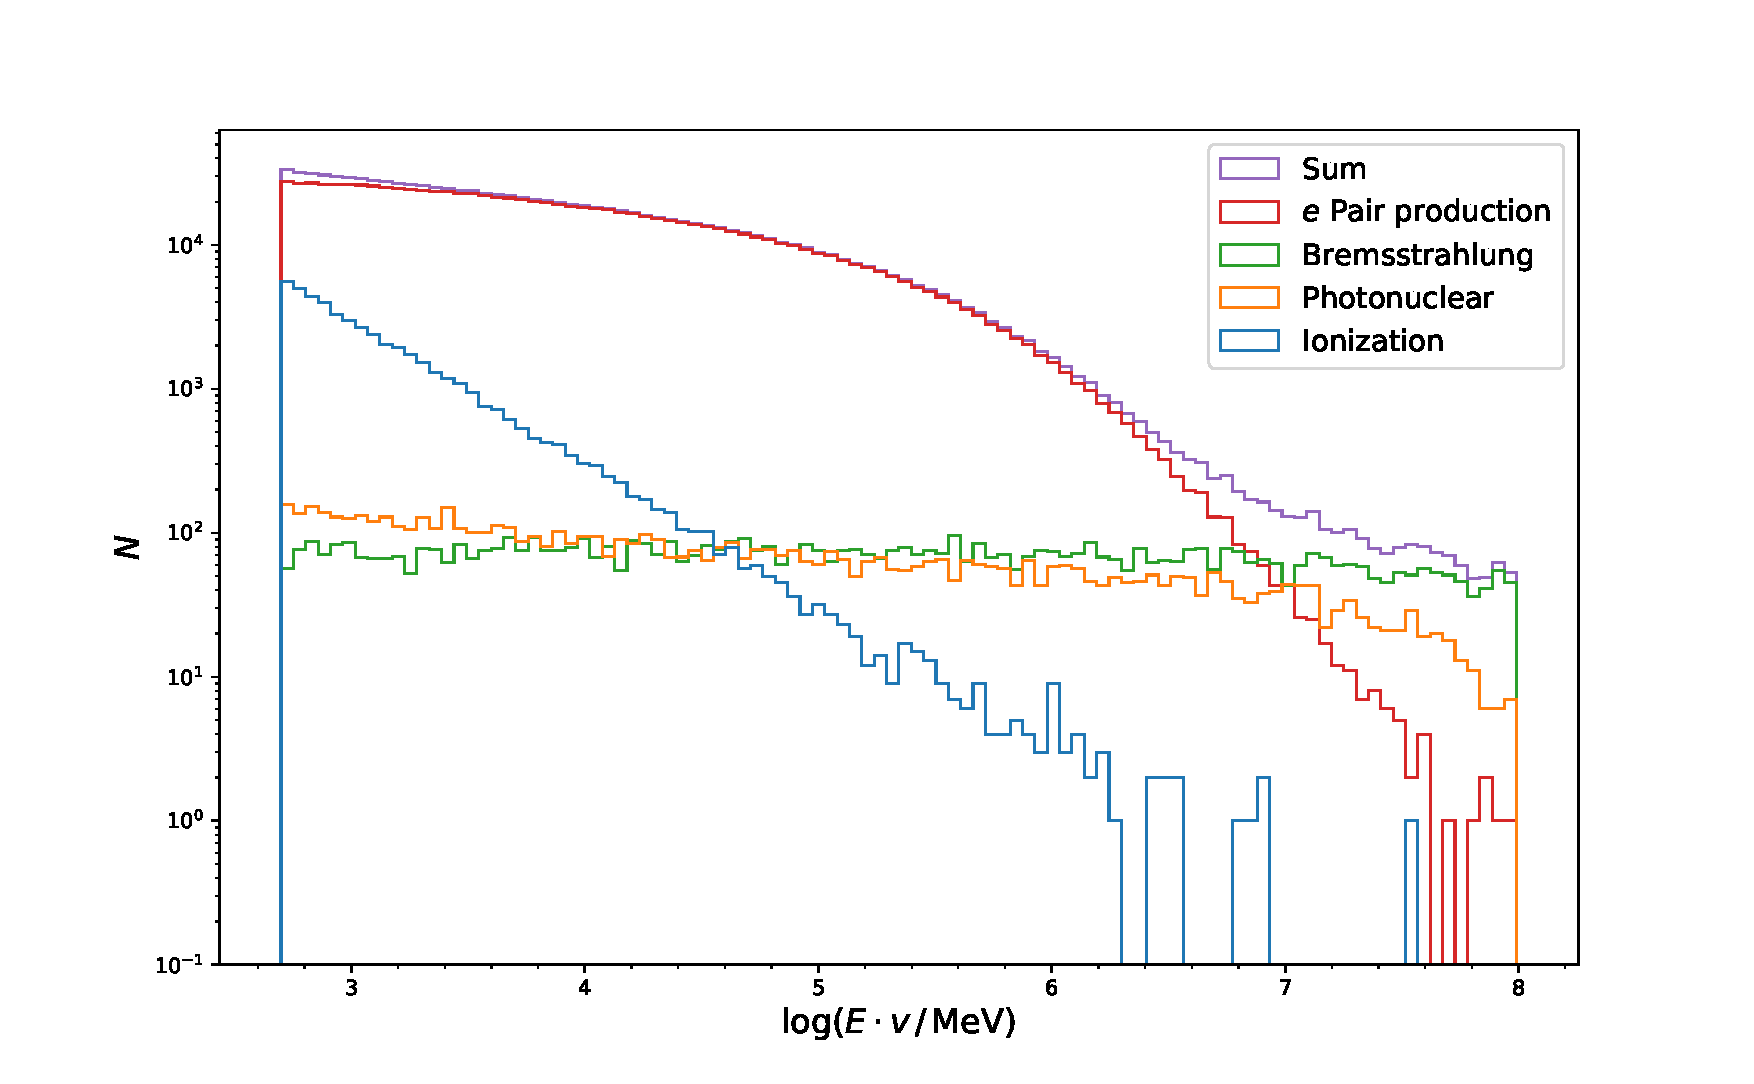
\includegraphics[width=\textwidth , trim=1.9cm 0.5cm 1.9cm 2cm,clip=true]{plots/standard.pdf}
  \end{minipage}\hfill
  \begin{minipage}[c]{0.3\textwidth}
    Propagation of $\num{e4}$ muons with energy $\SI{e8}{\mega\electronvolt}$ through $\SI{100}{\metre}$ of Standard Rock.
     \label{fig:03-03}
  \end{minipage}
\end{figure}

\end{frame}

%%% Muon pair prodction

\begin{frame}{Direct Production of Muon Pairs}
  \begin{columns}
    \column{0.5\textwidth}
    \begin{center}
      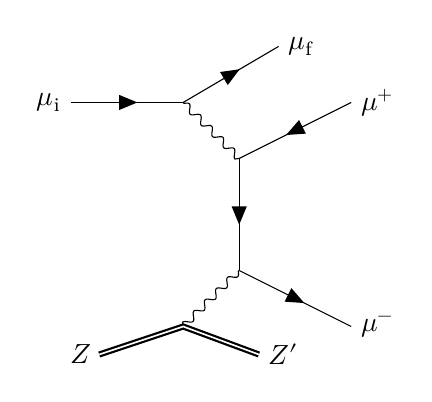
\begin{tikzpicture}
      \centering
       % Sizes
       \pgfmathsetmacro{\len}{0.05cm}
       \pgfmathsetmacro{\halflen}{\len/4}
       \pgfmathsetmacro{\vertexsize}{\len/20}
       \begin{feynman}
           % vertices
           \vertex (a) at (0, 0);
           \vertex (b) at (0, -1*\len);
           \vertex (d) at (-0.5*\len, 0.5*\len);
           \vertex (c) at (-0.5*\len, -1.5*\len);
           \vertex (i1) at (-1.5*\len, 0.5*\len);
           \vertex (i2) at (0, 1.5*\len);
           \vertex (f1) at (\len, 0.5*\len);
           \vertex (f2) at (\len, -1.5*\len);
           \vertex (f3) at (0.5, 1*\len);
           \vertex (z1) at (-1.25*\len, -1.75*\len);
           \vertex (z2) at (0.25, -1.75*\len);
     
           % draw diagram
           \diagram* {
             (i1) -- [fermion] (d) -- [fermion] (f3),
             (d) -- [boson] (a),
             (f1) -- [fermion] (a),
             (a) -- [fermion] (b),
             (b) -- [fermion] (f2),
             (b) -- [boson] (c),
           };
           \draw[thick, double] (z1) -- (c) -- (z2);
     
           % labels
           \node[left] at (i1) {$\mu_\text{i}$};
           \node[right] at (f3) {$\mu_\text{f}$};
           \node[right] at (f1) {$\mu^+$};
           \node[right] at (f2) {$\mu^-$};
           \node[left] at (z1) {$Z$};
           \node[right] at (z2) {$Z'$};
      \end{feynman}
    \end{tikzpicture}
  \end{center}
  \column{0.5\textwidth}
    With the energy fraction transferred to the muon pair:
      \begin{align*}
        v = \frac{\left( \epsilon_+ + \epsilon_- \right)}{E} \\[0.1cm]
      \end{align*}
    With the asymmetry parameter:
    \begin{align*}
      \rho = \frac{\left( \epsilon_+ - \epsilon_- \right)}{\left( \epsilon_+ + \epsilon_- \right)} \\[0.1cm]
    \end{align*}

    $E$: Initial energy of the ingoing muon $\mu_\text{i}$ \\
    $\epsilon_\pm$: Energy of the produced (anti)muon

  \end{columns}

\end{frame}

\begin{frame}{Double-differential cross section}

For production of muon pairs \footnote{Kellner, Kokoulin, Petrukhin: Phys. of Atomic Nuclei, Vol. 63, No. 9, 2000, pp. 1603-1611}:
\begin{align*}
  \frac{\mathrm{d}\sigma}{\mathrm{d}v \mathrm{d}\rho} &= \frac{2}{3\pi} (Z \alpha r_\mu)^2 \frac{1-v}{v} \Phi(v, \rho) \ln \left( X \right)
\intertext{%
For production of electron-positron pairs \footnotemark:}
  \frac{\mathrm{d}\sigma}{\mathrm{d}v \mathrm{d}\rho} &= \frac{2}{3\pi} Z \left(Z + \xi \right) \left( \alpha r_e \right)^2 \frac{1-v}{v} \left( \Phi_e + \frac{m_e^2}{m_\mu^2} \Phi_\mu \right)
\end{align*}
%$Z$: Kernladungszahl\\
%$\alpha$: Feinstrukturkonstante\\
%$r$: Klassischer Radius Elektron/Myon\\
\footnotetext{Kokoulin, Petrukhin: Proceedings of 12th ICCR, 1971, p. 2436}

\end{frame}

\begin{frame}<presentation:0>[noframenumbering]{Differential cross section}

\begin{figure}
    \centering
    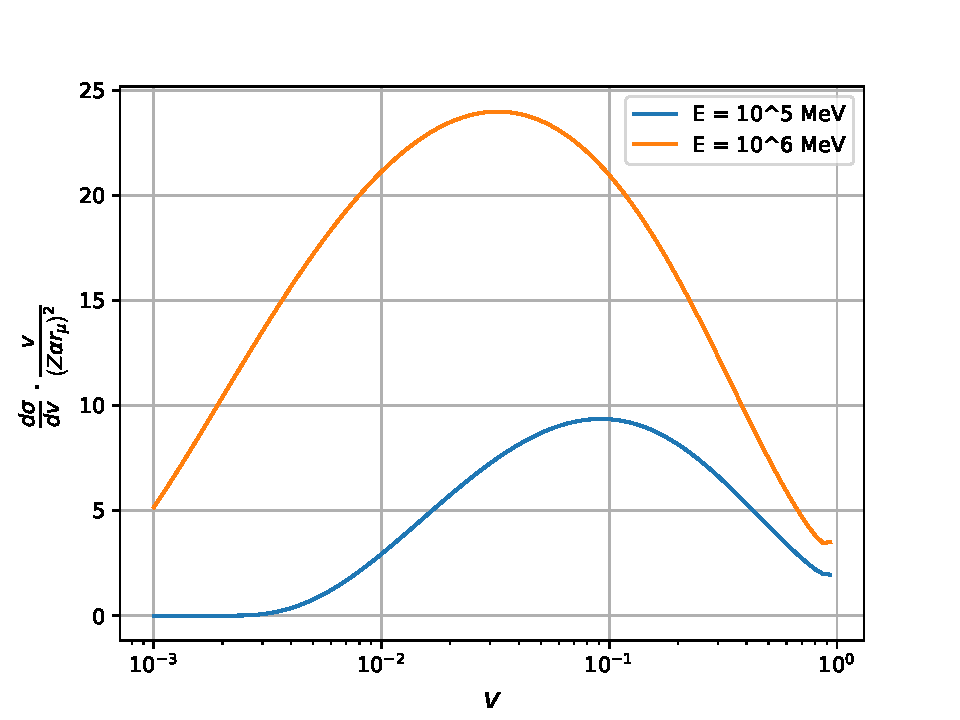
\includegraphics[height=0.8\textheight, trim=0cm 0.2cm 0cm 1cm,clip=true]{plots/mupair_crosssection.pdf}
    \caption{Differential cross section in $v$ for two different muon energies. Propagation in Standard Rock.}
    \label{fig:1}
\end{figure}

\end{frame}


\begin{frame}
\vspace{-5mm}
  \begin{columns}
    \column{0.4\textwidth}
Continous energy loss per distance
\begin{align*}
  - \left\langle \frac{\mathrm{d}E}{\mathrm{d}x} \right\rangle &= E \frac{N_\text{A}}{A} \int_{v_\text{min}}^{v_\text{cut}} v \frac{\mathrm{d}\sigma}{\mathrm{d}v} \mathrm{d}v
\intertext{%
with}
v_\text{min} &= \frac{2 m_\mu}{E}, \\
v_\text{max} &= 1 - \frac{m_\mu}{E}. \\
\end{align*}
    \column{0.6\textwidth}
\begin{figure}
    \centering
    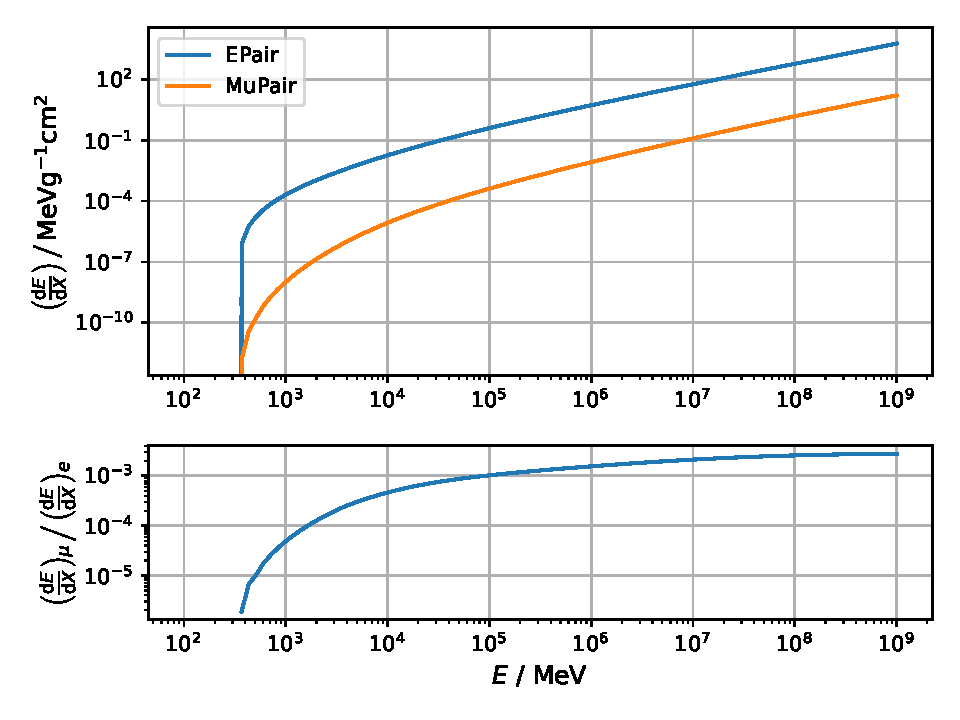
\includegraphics[height=0.85\textheight, trim=0.5cm 0.5cm 0.4cm 0cm, clip=true]{plots/mupair_compare.pdf}
    \caption{Comparion of $e$-pair and $\mu$-pair production, only continous losses (i.e.\ $v_\text{cut} = v_\text{max}$).}
    \label{fig:2}
\end{figure}
  \end{columns}

\end{frame}

\begin{frame}
\vspace{-5mm}
  \begin{columns}



    \column{0.62\textwidth}
\begin{figure}
    \centering
    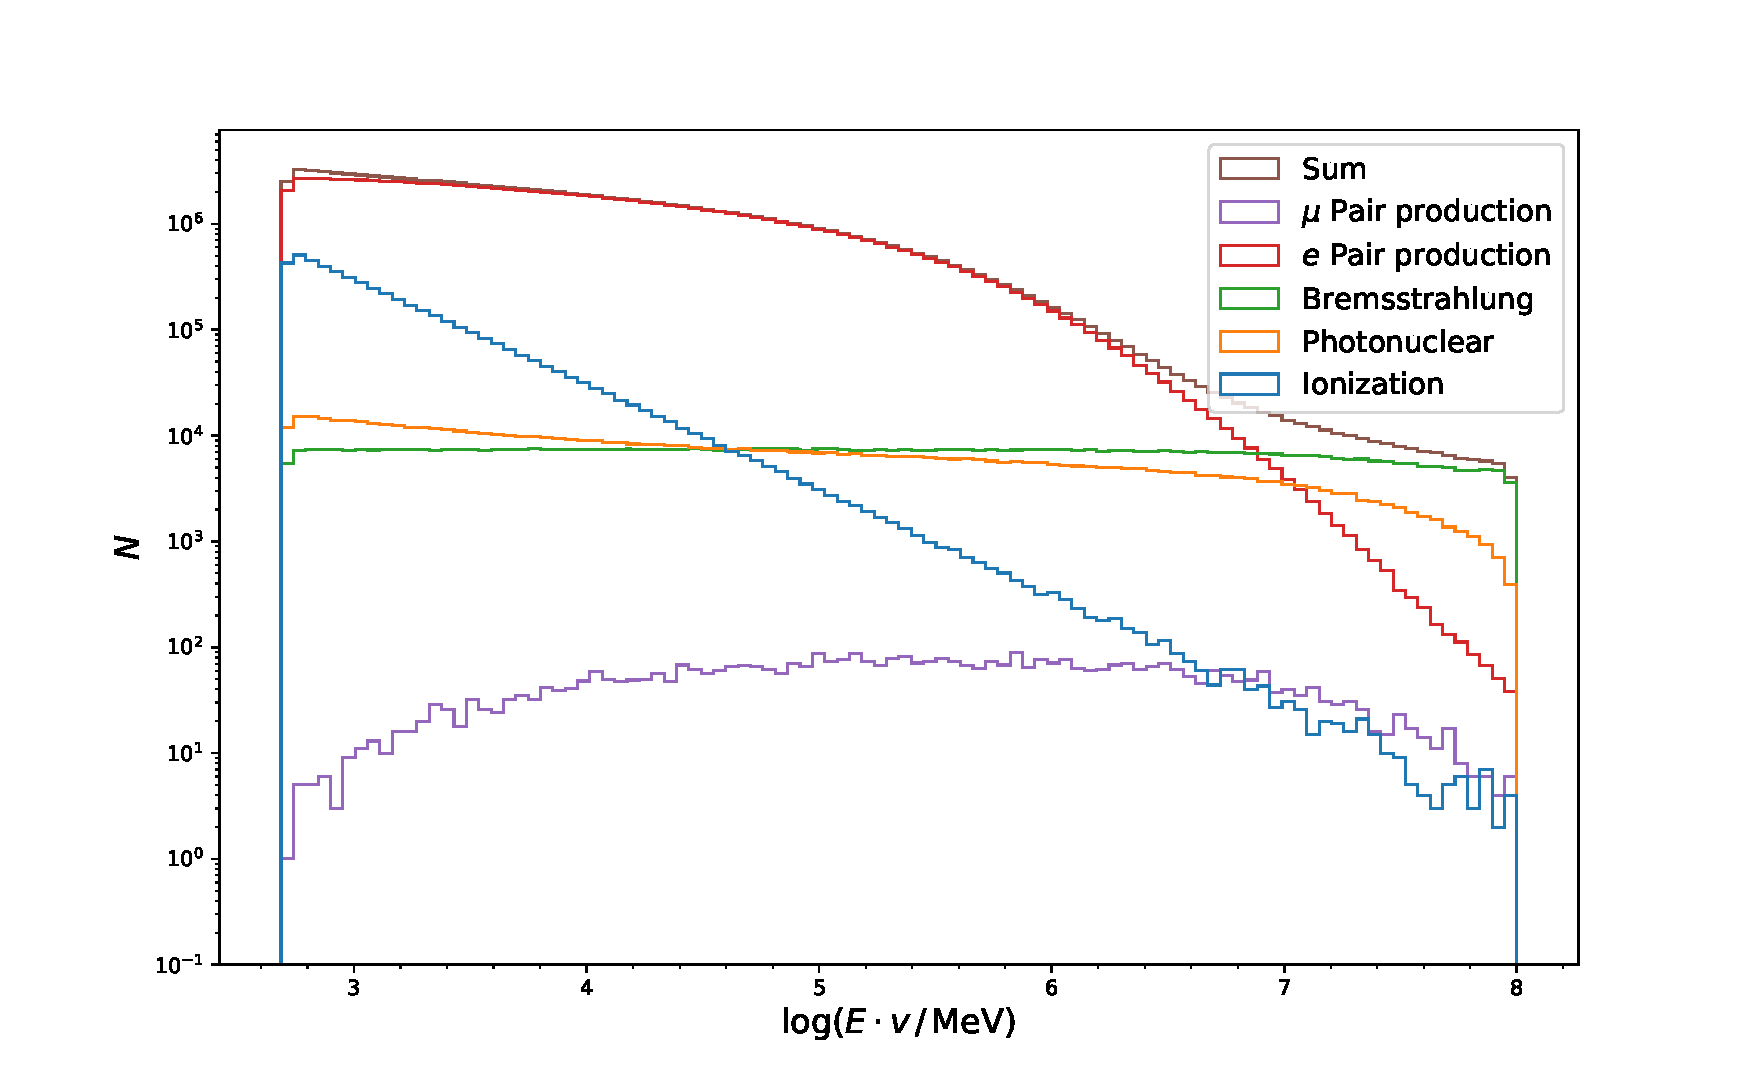
\includegraphics[height=0.8\textheight, trim=1.9cm 0.5cm 2.9cm 2cm, clip=true]{plots/mupair_secondaries.pdf}

    \label{fig:2}
\end{figure}

    \column{0.32\textwidth}
    \small
    \begin{table}
      \centering
      \begin{tabular}{c c c}
        \toprule
        $\text{process}$ & $N \,/\, N_\text{ges}$ & $E \,/\, E_\text{ges}$ \\
        \midrule
        $e$ pairp. & \num{0.94} & \num{0.94} \\
        Ionis. & \num{4e-2} & \num{5e-2} \\
        Brems. & \num{1e-2} & \num{7e-3} \\
        Photon. & \num{8e-3} & \num{6e-3} \\
        $\mu$ pairp. & \num{6e-5} & \num{5e-5} \\
        \bottomrule 
      \end{tabular}
    \end{table}

  \end{columns}
  \small
    \vspace{5mm}
    Stochastic losses in Standard Rock of \num{e6} muons with $E = \SI{e8}{\mega\electronvolt}$, $e_\text{cut} = \SI{500}{\mega\electronvolt}$, $v_\text{cut} = \num{5e-2}$.
\end{frame}

\begin{frame}
\vspace{-3mm}

\begin{figure}
    \centering
    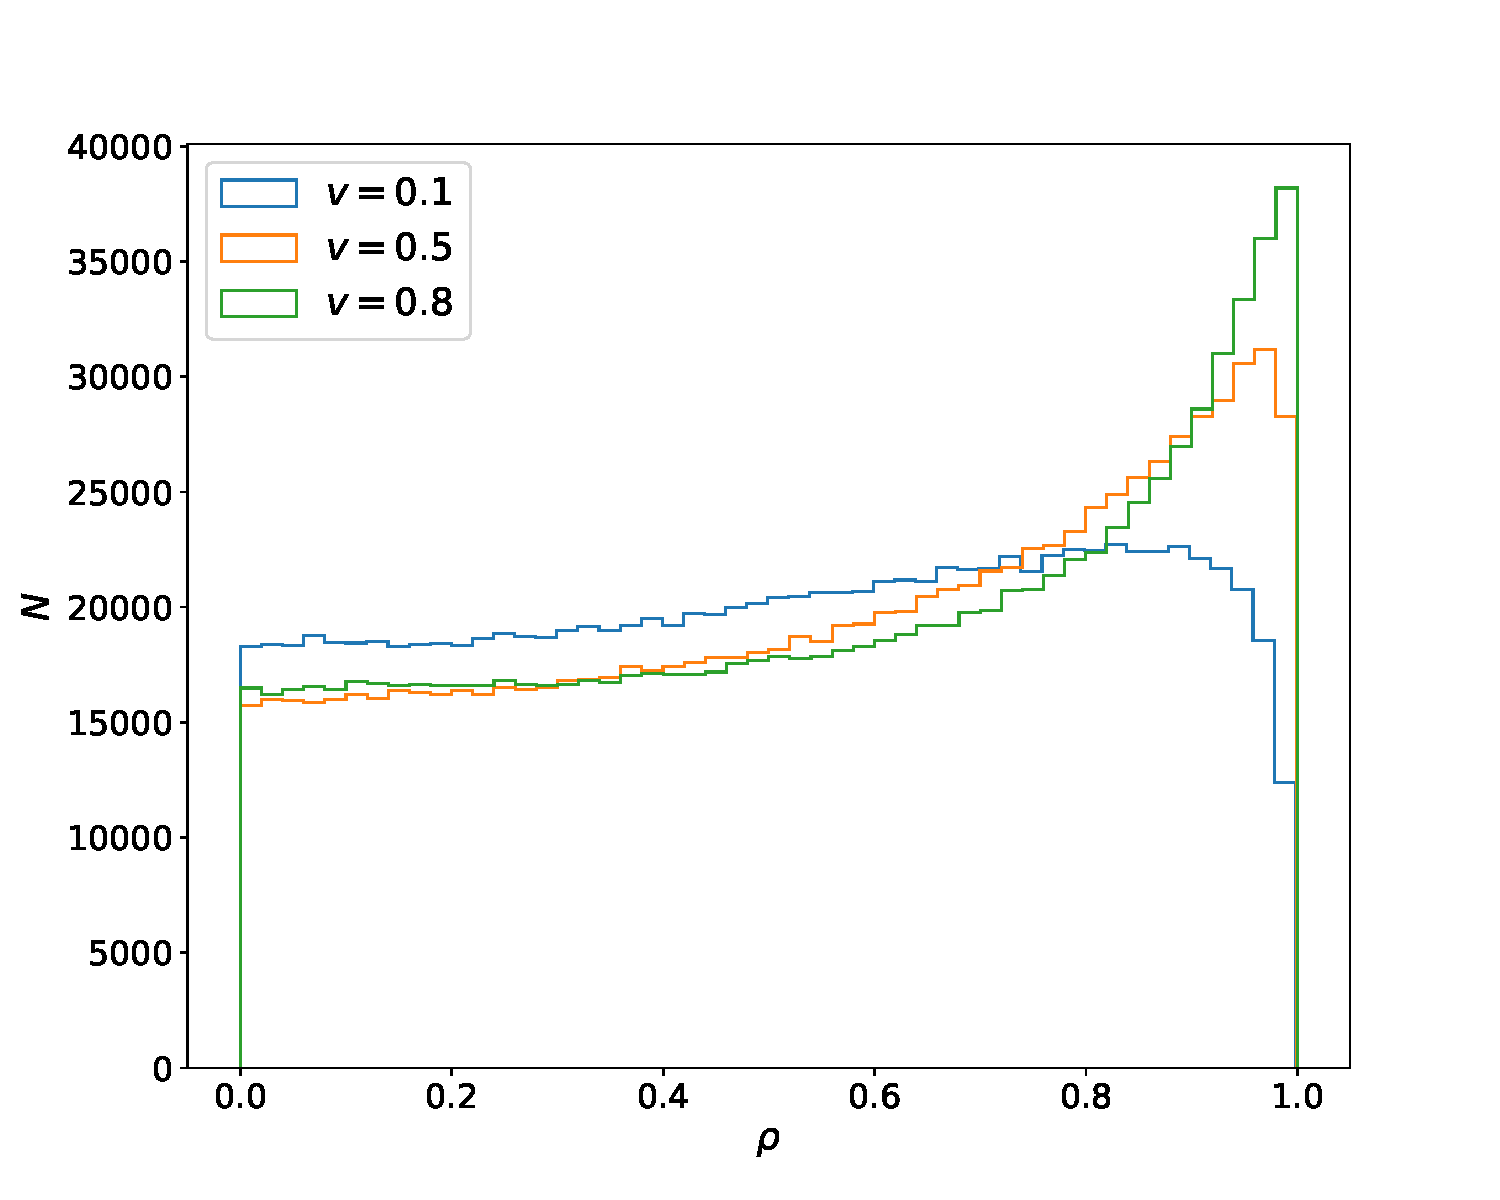
\includegraphics[height=0.9\textheight, trim=0.3cm 0.5cm 0.3cm 2cm,clip=true]{plots/plot_01.pdf}
    \caption{Sampling of $\rho$ for muons with $E = \SI{1e6}{\mega\electronvolt}$ and different $v$ in Standard Rock.}
    \label{fig:1}
\end{figure}

\end{frame}

%%% Weak interaction %%%

\begin{frame}{Weak interaction}
  \begin{columns}
    \column{0.5\textwidth}
    \begin{center}
      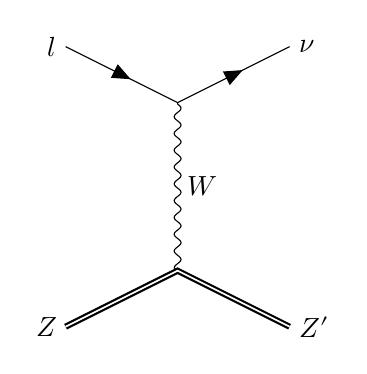
\begin{tikzpicture}
      \centering
       % Sizes
       \pgfmathsetmacro{\len}{0.05cm}
       \pgfmathsetmacro{\halflen}{\len/4}
       \pgfmathsetmacro{\vertexsize}{\len/20}
       \begin{feynman}
           % vertices
           \vertex (a) at (-1*\len, 0.5*\len);
           \vertex (b) at (0, 0);
           \vertex (c) at (1*\len, 0.5*\len);
           \vertex (d) at (0, -1.5*\len);
           \vertex (e) at (-1*\len, -2*\len);
           \vertex (f) at (1*\len, -2*\len);
     
           % draw diagram
           \diagram* {
             (a) -- [fermion] (b) -- [fermion] (c),
             (b) -- [boson, edge label=\(W\)] (d),

           };
           \draw[thick, double] (e) -- (d) -- (f);
     
           % labels
           \node[left] at (a) {$l$};
           \node[right] at (c) {$\nu$};
           %\node[right] at (f1) {$\mu^+$};
           %\node[right] at (f2) {$\mu^-$};
           \node[left] at (e) {$Z$};
           \node[right] at (f) {$Z'$};
      \end{feynman}
    \end{tikzpicture}
  \end{center}
  \column{0.5\textwidth}
    \begin{itemize}
      \item Highly suppressed process
      \item Similarities with "lollipop" signature in $\tau$-events
      \item Crossing symmetry \footnotemark:
      \begin{align*}
        \mathrm{d}\sigma\left( \mu Z \rightarrow \nu_\mu Z \right) = \frac{1}{2} \mathrm{d}\sigma\left( \nu_\mu Z \rightarrow \mu Z \right)
      \end{align*}
    \end{itemize}

  \end{columns}
  \footnotetext{Sandrock, Alexander: Higher-order corrections to the energy loss cross sections of high-energy muons, 2018, pp. 38-40}
\end{frame}

%%% Future %%%

\begin{frame}{Future: Physical improvements in PROPOSAL}
      \begin{itemize}
        \setlength\itemsep{0.5em}
        \item Improvement of electron/positron propagation
        \item Propagation of high-energy photons
        \item Deflection of particles in magnetic fields
        \item Allow continous density corrections in media
      \end{itemize}
\end{frame}

\end{document}
